\documentclass{report}
\usepackage{graphicx}
\begin{document}

%-------------------------------------------------------------------------------
%    TITLE PAGE
%-------------------------------------------------------------------------------

\begin{titlepage}
\newcommand{\HRule}{\rule{\linewidth}{0.5mm}}
\center
\textsc{\LARGE Imperial College London} \\[0.5cm]
\textsc{\Large Department of Computing} \\[0.5cm]
\textsc{\large BEng Individual Project} \\[1.5cm]
\HRule \\[0.3cm]
{\huge \bfseries LOST: \\[0.2cm] The Logic Semantics Tutor} \\[0.3cm]
\HRule \\[1.5cm]

% author and supervisors
\begin{minipage}{0.4\textwidth}
\begin{flushleft} \large \emph{Author:} \\
 Alina  \textsc{Boghiu}
\end{flushleft}
\end{minipage}~
\begin{minipage}{0.4\textwidth}
\begin{flushright} \large \emph{Supervisor:} \\
 Ian \textsc{Hodkinson}
\end{flushright}
\begin{flushright} \large \emph{Second marker:} \\
 Fariba \textsc{Sadri}
\end{flushright}
\end{minipage}\\[4cm]
{\large \today}\\[3cm]
\vfill
\end{titlepage}

%-------------------------------------------------------------------------------
%    ABSTRACT
%-------------------------------------------------------------------------------

\begin{abstract}
The aim of this project was to develop a software tool that can teach the 
semantics of first order predicate logic to students by helping them visualise 
the process of sentence evaluation. Thus, the focus was on developing an 
intuitive and engaging user interface to show and allow modification of 
structures, signatures and sentences, as well as provide relevant exercises for 
the student to practice with. The latter is arguably the most important feature 
of this tool and an addition to the functionality of the previous LOST projects. 
The user can now ask to see a number of questions. Completing each question is 
an actual achievement and provides real confirmation of understanding the 
semantics of first order logic. 
\\ \\
I believe these are firm grounds for many possible extensions (such as a
Hintikka game) and can be of real use, standalone or alongside the first year
predicate logic course. This report will provide further detail of its 
implementation and purpose.
\end{abstract}

%-------------------------------------------------------------------------------
%    ACKNOWLEDGEMENTS
%-------------------------------------------------------------------------------

\subsection*{\centering Acknowledgements}
I would like to express my gratitude and appreciation to \emph{Ian Hodkinson}, 
my supervisor, for his continuous support and motivation that have guided me 
towards completing this project, as well as to my second marker, \emph{Fariba
Sadri}, for her useful remarks and suggestions.
\\ \\
Altogether, the resources, staff and students of the Department of Computing 
have made working on this project enjoyable every day.

%-------------------------------------------------------------------------------
    \tableofcontents
%-------------------------------------------------------------------------------

%-------------------------------------------------------------------------------
%   INTRODUCTION
%-------------------------------------------------------------------------------

\chapter{Introduction}

LOST stands for LOgic Semantics Tutor and aims at providing students with a 
helpful tool for learning the semantics of first order predicate logic.

\section{Motivation and relevance}
First order logic is a powerful tool, of great importance in computing, 
mathematics and really any system relying on proofs. For students it is a way of
practising and developing important logical skills, it provides a formal mean 
for studying and understanding common mathematical structures and it forms a 
rigorous mind. However it is difficult for most students to learn the semantics 
of first order logic and with this being the key to assigning a truth value to 
any first-order logical sentence, the issue is important. This project attempts 
to provide a simple software solution and a solid base for future extensions. 
\\ \\
On the current market, there are a considerable number of tools designed to help
teach natural deduction or equivalences, but very few attempts have been made 
to design something that will accompany the student in learning the semantics 
of first order logic and even fewer of them are free. 
\\ \\
Feedback is currently restricted to lectures and tutorials which means this kind 
of instant guidance provided by computer software would make a great impact in 
the way students learn, improving both their and the teacher's experience. 
Designing such a tool raises interesting questions of what would make an 
interface intuitive and what does it need to provide the user with, such that 
they can learn and experiment with the semantics of first order predicate logic.

\section{A brief, non-technical description}
After a bit of thought and research into current solutions, I realised it would 
not be easy to implement in an attractive way and this will become more obvious 
after discussing the existing work. Thus one of my guidelines shaped up to be 
engaging the student as much as possible which software can do if it is 
intuitive, bug free and most importantly rewarding. 
\\ \\
The first of these would be achieved if the user is allowed to naturally 
interact with the application. Because in reality no one likes to read manuals, 
I aimed to make my program safe to use with a ``click and see what happens'' 
approach. This required reasoning about as many occurable events and exceptions 
as possible. 
\\ \\ 
As for the actual content point of view, it would be useful if the user 
could visualize structures in such a way that they could easily guess the 
meaning of a possible sentence within it. They should be able to use a 
toolbox-like signature representation to add and remove objects and relations as 
well as have a way of introducing and evaluating sentences. At this point it 
became clear that the interface would have three main aspects to handle: 
structures, signatures and sentences, which will be discussed further in the 
implementation details section. 
\\ \\
Next, I aimed for a solid back end that could handle even a completely different 
interface implementation. This meant for it to be able to correctly evaluate the 
semantics of a logic formula given a structure, regardless of the input or 
output method. Parsing the input sentence (be it from a terminal or a GUI) would 
therefore have to be done reliably and its representation in memory be clear, 
effectively accessible and easy to evaluate. 
\\ \\
Features described so far would constitute a minimum viable product, however 
making it such that the student feels their time was spent worthily was just as 
important. I aimed to achieve this by implementing a simple quiz system with the 
possibility of further development. This particular functionality would provide 
the confirmation a student needs when asked to learn anything.

\section{Report Overview}
In the following chapters the reader can expect a walk through the process of 
developing the final product, from gathering background information to 
implementation details, testing procedures and, an as much as possible honest 
evaluation of the outcome. 
\\ \\
Though previous knowledge of first order predicate 
logic and Java would help in understanding the effort that went into this 
project and its relevance, it is not compulsory. I will revise the essential 
aspects of the theoretical side\cite{logicslides}, however basic knowledge of 
logic operators and their meaning (i.e.\ and, or, implies etc.) is assumed.

%-------------------------------------------------------------------------------
%   BACKGROUND
%-------------------------------------------------------------------------------

\chapter{Background}

\section{First order predicate logic semantics}
In order to understand the product I am aiming for we should first take a look 
at what first order predicate logic is and why its semantics can be tricky. As 
an extension of propositional logic, it expresses statements such as \emph{
Socrates is a man} in much more detail. While propositional logic would regard 
this sentence as atomic and simply assign it a truth value, predicate logic 
provides a way of describing its internal structure and of evaluating it within 
a relevant context. I will use this sentence to briefly introduce the key 
concepts used in predicate logic to make ``splitting the atom'' possible. 
These are:

  \begin{itemize}
  \item \emph{Constants} 
  - which name the objects inside a context (e.g.\ Socrates). One constant can 
  name exactly one object.
	\item \emph{Relation symbols}
  - which describe properties of the objects they take as arguments or, in the
  case of nullary relations (which take no arguments), general properties of the
  structure (e.g.\ \emph{man} is a unary relation, it represents a property that 
  Socrates may or may not have).
  \end{itemize}

\noindent In order to keep track of these two new concepts, we use a \emph{
signature}. This represents the syntactic side of evaluating a sentence and 
provides the necessary tools: constant names and relations symbols. For a 
computer scientist it may be easier to look at it as a collection of abstract 
classes that can be instantiated to form the structure and give it meaning.
\\ \\
Using just these concepts, we can now rewrite the sentence we discussed as 
\emph{man(Socrates)}. However we still cannot decide its truth value and at this
point two questions arise: First, which is the object that Socrates describes?
Second, what does it mean for something to be a man?
\\ \\
This is where the \emph{structure} comes in. It is defined to be a non-empty set
of objects that the signature knows about. If we take our structure to be an
imaginary world of hobbits and name one of them Socrates, our sentence would be
false, as Socrates would not be a man, he would be a hobbit. However in the 
context of the real world where Socrates names the famous philosopher, the 
sentence is true. 
\\ \\
Next, if we want to express something like \emph{All men are mortal} we must 
introduce the two quantifiers. Again, these can be viewed as a way to iterate 
over the objects that form a structure. These are:

	\begin{itemize}
	\item \emph{$\exists$ (Exists)} 
  - which checks that there is at least one object in the structure that
  satisfies the sentence it refers to and makes it true.
	\item \emph{$\forall$ (For all)}
  - which checks that all of the objects in the structure satisfy the sentence 
  it refers to and each make it true.
	\end{itemize}

\noindent The sentence can now be written as
\emph{$\forall$(man(x) $\rightarrow$ mortal(x))}
and we refer to x as a bound variable because it is pinned down by a quantifier,
in this case $\forall$. A more precise reading of the above formula would be:
"If something is a man than it is mortal." 
\\ \\
Another aspect that the user must understand is that sentences containing 
unbound variables are also valid but cannot be evaluated to a truth value. 
Saying "men(x) $\rightarrow$ mortal(x)" makes no sense until we decide what x 
refers to. If x were a constant than it would refer to the object it names, 
however common practice dictates that we reserve the last letters of the 
alphabet for naming variables. It is this kind of subtlety that I am hoping
to make clearer with the help of an interface which shows exactly which objects
are named by constants and which can only be referred to by using quantified 
variables. 
\\ \\
The theoretical side is obviously what forms the base of this project. It is 
therefore natural that the implementation follows its key aspects: the 
structure, the signature and the logic formulas. Throughout the report I will 
inevitably make references to the concepts summarised in this section whilst 
possibly making further additions and clarifications.

\section{Existing solutions}
As mentioned before, previous attempts have been made to provide software 
solutions to teaching predicate logic semantics. In fact one student provided a 
solution for this same project specification in 2007. Furthermore, the Openproof
Project at Stanford's Center for the Study of Language and Information (CSLI) 
is concerned precisely with the application of software in logic and they have 
developed Tarski's World for this purpose.

\subsection{LOST 2007}
This application was previously available on the DoC's lab machines. Currently 
however, the only available resource is the user manual. As it is a solution to 
the same project specification I have carefully studied it and picked up what I 
thought were several good ideas, whist taking note of things I should avoid.

\begin{figure}[h!]
\centering 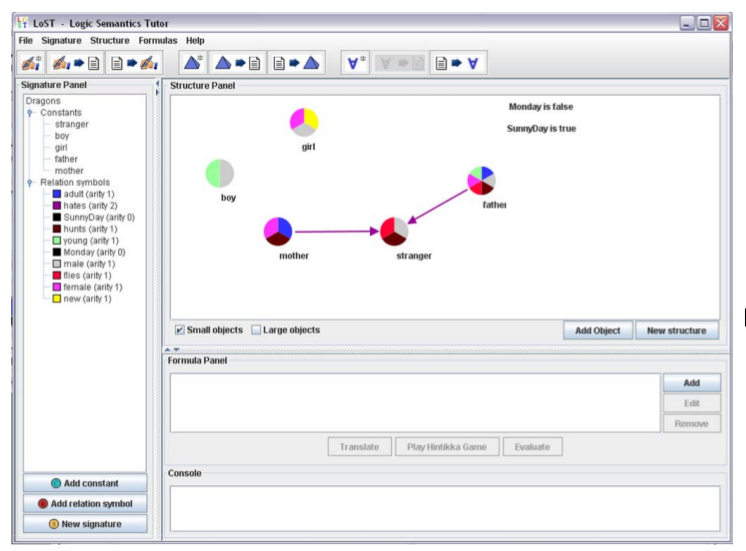
\includegraphics[scale=0.4]{oldlost.png}
\end{figure}

\noindent The application provides a good representation of the logical 
structure. It displays objects as circles, filled with colours corresponding to 
the unary relation symbols that apply. Binary relation symbols are represented 
as arrows, also colour coded. The user can drag objects to rearrange them as he 
seems fit. This representation is quite clear and easy to interpret. For this 
reason my own implementation is similar, with a few changes aimed at smoothing 
the experience even further. 
\\ \\
First I decided objects should have a clear base colour 
displaying only their name in the case of constants. Then, according to which 
unary relations apply to it, coloured borders would be added or removed. This 
eliminates the risk of a confusing pie chart when an object has many relations 
referring to it. Next, the arrows would be labelled with a list of names of the 
relations they represent, such that if multiple relations exist amongst two 
objects there is no need for multiple arrows rendering better space efficiency.
\\ \\
Furthermore the application allows the user to interact with the structure with 
several buttons, a signature tree and a number of forms for creating structures 
and introducing formulas for evaluation. These are offered to the user according 
to their intention. The general purpose of all this is important and the 
functionality essential to the application. However in my own implementation I 
tried to minimise the number of buttons and additional windows or forms, keeping 
it simple and in one place. 
\\ \\
Finally the application offers the possibility to play a Hintikka game, which is 
a wonderful way of practising logic semantics skills. It also makes an attempt 
at logic to English translation. These would make very useful extensions to my 
own application as I chose to focus on the tutorial aspect.

\subsection{Tarski's World}
The Tarski's World\cite{tarski} application is based on the same principle. Its 
representation of the structure is a 3D world of blocks. It uses an interpreted 
first-order language which allows users to write sentences about the world and 
evaluate their truth. A Henkin-Hintikka game is also provided, along side the 
main game which consists of questions about the active sentences. This was 
useful when implementing my own tutorial questions. 

\begin{figure}[h!]
\centering 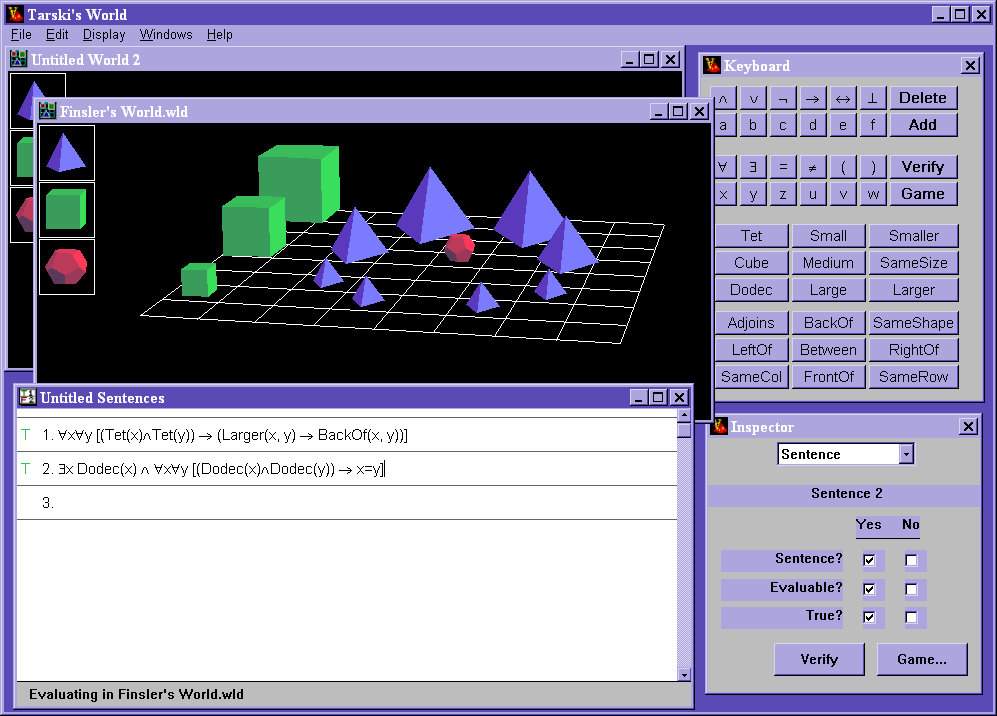
\includegraphics[scale=0.3]{tarski.png}
\end{figure}

\noindent My single reservation was once more the number of menus, panels and 
buttons (as seen in the picture above) that can become quite irritating since 
only a few are truly relevant and most don't seem worth the effort of figuring 
out. From the point of view of a student this can be quite off putting and might 
drive them towards the classic pen and paper approach. Otherwise it is generally 
very professionally made and I did not encounter any major flaws. The learning 
experience is complete if we take into account the extensions including text 
books and an online evaluation system that grades the student's performance 
which I particularly appreciated.

\section{Ideas shaping the final approach}
After looking into the above mentioned solutions and others similar to them it 
became obvious that the main difficulty with providing a teaching tool for logic 
semantics is in fact teaching the student to use it. When working with these 
tools I got the feeling they let the back end lead the implementation of the 
interface instead of using the latter to hide the inner works. For example, just 
because there are say 20 relation symbols active in the signature does not mean 
the user wants to see them at all times in a big grid of buttons that takes up 
half of the work space. I believe it is important to let the user focus on 
semantics without having to worry too much about the syntactic aspect, which 
should be provided and hidden as much as possible. 
\\ \\
Another remark should be made on the tendency of developers to forget the user 
does not know as much as they do. It is impossible to develop a teaching tool 
without understanding first order predicate logic inside out, which makes it is 
even harder to empathise with a student that is just starting to learn it. It is 
therefore easy to unconsciously overestimate the user's knowledge and forget to 
provide explanations that might in fact be useful to them. For example it might 
seem counter intuitive that a sentence such as man(Socrates) is false. But if 
the signature's only unary relation symbol is \emph{hobbit} this may seem 
obvious to a logician. However the user who tried to input the above sentence 
might benefit from a message such as ``The unary relation symbol man is not 
defined in this structure'', instead of their sentence just being rejected as 
invalid without any notice.
\\ \\
Finally, I fixed the two features that would make this project unique. First of 
all I would keep it as simple as possible, making it a priority to minimise the 
number of buttons and choices the user has to make. This had to be done without 
sacrificing any of the essential functionality. Secondly, I would make it 
rewarding, by giving the user an opportunity of testing their skills. As several 
students have worked on this project specification across the years, I figured 
this would be a useful and fresh addition.

\section{Software choices}
Having sufficiently stressed the importance of the interface I had to make a 
choice as to which programming environment would best fit its requirements. I 
wanted to be able to focus on building something attractive without having to 
worry too much about the lower level issues like memory assignments, garbage 
collection or optimal for loop nesting. 
\\ \\
This, as well as my previous programming experience, 
perused me to choose Java 7\cite{javaAPI} and Swing\cite{javaTUT}, which 
proved to be at a high enough level for my interface whilst offering me 
the freedom to design the back end for the sentence evaluation from scratch. 
Thus I had complete control and understanding of every step that takes a 
sentence from it's raw form to an outcome. And understanding made it easier to 
track bugs, make changes and pursue a steady development. Java also ensures a 
decent compatibility across computer platforms, has extensive documentation and 
is a reliable language that addresses a large audience. 
\\ \\
Of further help with the the interface was the IDE. After starting off with 
Eclipse, I soon realised the simple task of arranging buttons on the panel was 
uselessly tedious. So after a little research I chose to use NetBeans for its 
GUI Builder. It took a bit of getting used to, especially with learning to get 
around the read-only generated code, but eventually everything proved to be 
100\% customisable and certainly worth switching to. Overall this saved me 
significant time and helped me achieve my desired esthetic standard. 
\\ \\
Java proved to be the right choice again when it came to writing a parser for 
the logic formulas. It made it easy to link an automated parser, reducing my 
task to writing a comprehensive grammar. At this point, another choice was to 
favour Antlr4\cite{antlr4} over the previous, better known version. What 
convinced me was its ability to deal with left recursive grammars. Although 
removing recursivity is a straight forward algorithm\cite{compilers}, it makes 
the grammar quite ugly and a bit more difficult to read. Antlr4 also uses an 
impressive adaptive parsing strategy, making it significantly more time 
efficient than its static ancestors.
\\ \\
For version control I used Git\cite{progit}. It is an easy and reliable way of 
keeping backups, working remotely, tracking progress and proved essential for a 
project this size as it happened more than once that I had to revert to previous 
commits and slowly add in changes to discover bugs. It also proved useful for 
its branches, allowing me to experiment with external Java packages such as 
mxgraph, and make other temporary changes.
\\ \\
For the report I used LaTeX\cite{latex} with Vim, which greatly facilitated the 
text formatting and made it easy to keep track of the different sections. The 
Unix shell was also of great use with compiling Antlr and LaTeX and using 
Git as well as with occasional remote connections. Finally, the entire project 
was developed on a Ubuntu 12.04 system.

\section{Design Patterns}
As developing proceeded, the size of the code became overwhelming. The 
separations packages and classes provided was insufficient. When it came to 
implementing the smallest changes, dependencies inside the code made it a 
tedious and time consuming task. Therefore, when the back end was finished and I 
began developing the user interface, I took a step back and revised some 
software design patterns, in order to choose a system that would best fit my 
requirements. 
\\ \\
It was the \textbf{Model-View-Controller} pattern that helped the most. By 
completely separating the back end from the display I was able to keep better 
track of the whole picture:
\begin{itemize}
\item Model - this represents everything in the back-end. It handles all the 
information concerning sentences, signatures, structures and evaluation. 
\item View - this represents the interface. It contains all the component 
types needed to represent logic objects. It also handles the display layout and 
appearance and contains the project's main method.
\item Controller - this is the class that links the model to the view. To do 
this it pairs up logic objects with an appropriate graphical component. It also 
interprets user input such that it can be sent back to the model for 
interpretation. 
\end{itemize}
Having separated the information from the representation in this way, it became 
much easier to change the interface since I no longer had to worry about the 
compatibility with the model. This was essential as designing the GUI meant 
repeatedly using the application and applying slight variations to see what 
would be most comfortable for the user. 
\\ \\
I also used the \textbf{Adaptor} structural design pattern, which allowed me to 
separate the parser generating from the sentence structure. I then used an the 
Sentence class constructor to convert the parse tree into my own logic tree, 
which I had designed with an integrated evaluator. 
\\ \\

%-------------------------------------------------------------------------------
%   MAIN BODY
%-------------------------------------------------------------------------------

\chapter{Approach and Implementation details}

This logic semantics tutoring tool is naturally shaped around the theoretical 
elements that provide logic formulas with meaning. It contains three packages 
which I will discuss in the same order they were developed:

  \begin{itemize}
  \item Evaluator - that holds the logic tree structure along with an adaptor 
  for the parse tree and an evaluator.
  \item Parser - which handles the translation of raw logic formulas input as 
  strings into a parse tree.
  \item GUI - which contains the user interface and controller.
  \end{itemize}

\section{Evaluator}
As it can be deducted from the brief description above, this is the main and 
largest part of the software. I will start with how logic formulas are supported 
then move onto the evaluation process and finally the adaptor. 
\\ \\
The starting point of my project was representing sentences in an efficient 
computer readable format. It was also important to remain close to a human 
friendly representation. The solution came once from logic theory, where 
sentences are often represented with the help of logic trees. These trees have 
logic operators or quantifiers for nodes and simple atomic formulas for leaves. 
For example, the sentence \emph{$\forall$(men(x) $\rightarrow$ mortal(x))} is 
represented by the following tree:

\newpage
\begin{figure}[h!]
\centering 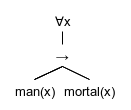
\includegraphics{mortal.png}
\end{figure}

\noindent So with this in mind the first step was to build the classes to 
represent the logic elements that would be used to form the nodes of the logic 
tree.

  \begin{itemize}
  \item NullaryRel, UnaryRel, BinaryRel \\
  Classes to represent relations symbols with arities from 0 to 2. Although it 
  is possible to have higher arities they are not common in predicate logic and 
  would over complicate the representation too much. Once a stundents 
  understands these three, relations of higher arities are merely an inductive 
  step away.
  \item Term \\
  A class to represent the parameters relation symbols take. It has a name and 
  is extended by Constant and Variable. The latter adds boolean fields 
  indicating whether it is bound by a certain quantifier. 
  \item BinOp \\
  An enum type containing all the binary logic operators along with definitions 
  of their behaviour (i.e.\ functions overriding the abstract function evaluate 
  using the Java logic operators).
  \end{itemize}

\noindent To ensure the correct result when comparing instances of these 
classes, I made sure to to override their default equals method appropriately. 

\subsection{Logic Tree}
Next I build the actual nodes. Each extends the abstract LogicTreeNode class, 
overriding the evaluate function and providing a pointer to the next node (or 
nodes in the case of binary operators). They are of course encapsulated by a 
LogicTree class which has the head of the tree to nicely call evaluate upon. 
Let us see how each node works in decreasing order of their complexity:

\begin{itemize}
\item ForAllNode\\
This node's evaluation function returns the boolean value representing whether 
each of the objects in the structures make the sentence true. And it is very 
important to understand the difference between each object making the sentence 
true and all objects making the sentence true. For example, to verify the 
sentence \emph{$\forall$x (men(x) $\rightarrow$ mortal(x))} (All men are mortal) 
we would take each man in turn and verify that he is mortal, disregarding any 
animals or other things. It would be wrong to first verify that everything is a 
man and if so, then verify that everything is mortal. Such a sentence would be 
written as \emph{$\forall$x men(x)$ \rightarrow \forall$x mortal(x)}. 
\\ \\
To make this even more clear, let us assume the structure contains an immortal 
man. This would make the first sentence false because not all men are mortal. 
However in the case of the second sentence, when verifying that everything is a 
man, we would find that is not true since there are also animals and other 
things in the structure. And since falsity implying anything is always true, the 
second sentence is true. Hence the two sentences have different outcomes and 
mean different things. 
\\ \\
In order to handle this correctly, the ForAll node passes an assignment down 
the tree to be evaluated with the entire sentence in scope. An assignment 
represents an object from the structure's domain. The class Assignment contains 
a Term and a Variable field to pair them. 
\\ \\
For each object in turn, the node adds one assignment to an array list
of assignments in case other quantifiers are encountered down the tree. 
This is used as a parameter by the evaluation function. Only when it has 
finished iterating over the structure's objects, it puts a final result 
together. If all of them verify the sentence then the final result is 
returned as true, otherwise as false. I will show the evaluation
functions here, and most of it will be relevant for the exists node as well:
\begin{verbatim}
@Override
boolean evaluate(Structure s){
    ArrayList<Assignment> assignments = new ArrayList<>();
    return evaluate(s, assignments);
}

@Override
boolean evaluate(Structure s,
                 ArrayList<Assignment> assignments){
    boolean outcome = true;
    for (Term t : s.terms) {
        Assignment a = new Assignment(t, var);
        assignments.add(a);
        outcome &= next.evaluate(s, assignments);
        assignments.remove(a);
    }
    return outcome;
}
\end{verbatim}
\newpage
\item ExistsNode\\
This node follows the same principle. The difference is outcomes of each 
assignment are put together with an or operator, such that as soon as one is 
found to be true, the evaluation stops and returns true. If however it reaches 
the end of the structure domain without finding a term to satisfy the sentence, 
it returns false.\\
At this point it must be clarified that there are in fact two abstract 
evaluation functions as follows:
\begin{verbatim}
abstract boolean evaluate(Signature s);
abstract boolean evaluate(Signature s, 
                          ArrayList<Assignment> assignments);
\end{verbatim}
This is because it may be the case that no quantifiers exist in the sentence. 
For example a sentence may only refer to constants.

\item BinaryRelNode and UnaryRelNode\\
This is a leaf node class and contains a BinaryRel field. The evaluation method 
checks that the structure contains the relation held in this field. If the 
relation's arguments are constant no assignments are involved. If however 
variables are involved, the second evaluation method is called and it creates a 
new relation with the relevant terms from the relevant assignments as arguments. 
This new relation is then checked against the structure. I believe the 
evaluation functions of the UnaryRelationNode class summarises this best:
\begin{verbatim}
@Override
boolean evaluate(Structure s) {
    return s.unaryRels.contains(rel);
}

@Override
boolean evaluate(Structure s, ArrayList<Assignment> assignemnts) {
    if (rel.arg instanceof Variable) {
        for (Assignment a : assignemnts) {
            if (rel.arg.equals(a.boundVar)) {
                UnaryRel r = new UnaryRel(rel.name, a.assignedTerm);
                return s.unaryRels.contains(r);
            }
        }
    }
    return this.evaluate(s);
}
\end{verbatim}

\item NullaryRelNode \\
This node has a NullaryRel field and always return's that relation's boolean 
value. Nodes such as this, that do not need an assignment to return a value,
do not alter the assignments, but simply pass them on.

\item EqualsNode \\
Although it may seem like it could be part of the BinOpNode, this node is 
actually a leaf as the equals operator takes terms for arguments. So really it 
is more similar to the BinOpNode. If the arguments are constants it checks that 
they are in fact the same object. If any of the arguments are variables it uses 
the assignments to look for appropriate terms (i.e. it replaces the variable 
with the assignedTerm field value of the assignment that has the same variable 
in its var field). It will help to see the Assignment class:
\begin{verbatim}
class Assignment {
    Term assignedTerm;
    Variable boundVar;

    public Assignment(Term t, Variable var) {
        this.boundVar = var;
        this.assignedTerm = t;
    }
}
\end{verbatim}

\item BinOpNode \\
This is an internal node containing one of the types of operators defined in the 
enum type described before, as well as pointers to the nodes it takes as 
arguments. Its evaluation function calls the evaluation functions of the these 
two nodes in the was described by the operator definition. For example AND will 
make sure the evaluation functions return true for both arguments.

\item NotNode \\
Also an internal node that points to the rest of the sentence through a 
LogicTreeNode field and simply returns its negated outcome.

\item TruthNode and FalsityNode \\
These node always return true and false respectively. They represent leaf nodes.

\item DummyNode \\
This node is used by the adaptor to translate parse trees an will be further 
discussed in the relevant section.
\end{itemize}

\subsection{Signature}
In order to understand the symbols used in the logic formula, a signature is 
needed. In a series of ArrayList fields it holds Strings representing names of 
the Constant, NullaryRel, UnaryRel and BinaryRel instances. In order to fill 
these in, its constructor takes a signature object as a parameter.
\\ \\
The choice for an array list (here and in other classes) was based on the fact 
that, being based on a dynamically resizeable array, it would greatly facilitate 
adding and deletion of objects as well as locating and iterating over its 
elements. 
\\ \\
Using just the relation symbols' and constants' names it provides another useful 
check of the formula's syntax before passing it on to the evaluator. If any 
symbol used in the sentence is missing from the signature and is not a 
quantified variable, the user will be prompted with the appropriate message. 
However this will be discussed further in the section regarding interface 
implementation where the signature's contribution is greater. In the evaluation 
context its role is simple: it checks that all the symbols used are declared 
and valid.

\subsection{Structure}
Now that we have seen the representation of a logic formula and signature, we 
can proceed to understanding the format of the context in which it will be 
interpreted. Objects constructed by the Structure class are passed as a 
parameter to the evaluation method such that an interpretation can be made. 
\\ \\
The fields of this class are array lists of terms and relations. In order to 
fill them in, the constructor calls a generate method. This in turn uses four 
enum types with names for constants and the three types of relations. Each enum 
type has a random chooser method to return one of its members. The generate 
method uses this and ensures no duplicates are allowed into the final content of 
the structure. It generates a random number of actual terms and relations using 
the Term, Constant, and relation class constructors described before. 
\\ \\
Every time the program starts up it creates a new structure which the user can 
modify, thus ensuring a non empty set of elements at all times to remain 
consistent with the theoretical definition. The details of this will be 
discussed in the user interface section.
\\ \\
The following UML diagram\cite{uml} summarises the structure and signature 
classes:
\newpage
\begin{figure}[h!]
\centering 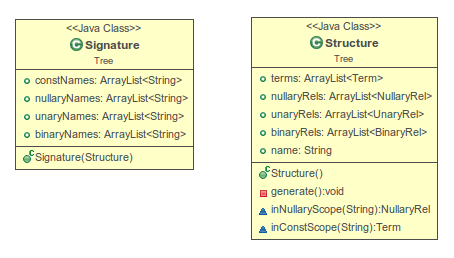
\includegraphics[width=\textwidth]{SnS.png}
\end{figure}

\section{Parser}
I have already discussed the choice of Antlr4 for the purpose of parsing a logic 
formula from plain string input. In order to generate a parse tree, Antlr needs 
two things: a grammar and lexer rules. 
\\ \\
\textbf{The grammar} has proved quite tricky to write as I wanted to offer the 
user as much input freedom as possible. I also managed to preserve the operator 
precedence such that it would make it easier for the adaptor to interpret the 
parse tree. The final and best solution was once more the simple one, with the 
main rule shaping to be comprehensive and easy to read:
\begin{verbatim}
formula
  : TRUTH
  | FALSITY
  | term EQUALS term
  | relation
  | quantifier formula
  | NOT formula
  | formula AND formula
  | formula OR formula 
  | formula IMPLIES formula
  | formula EQUIV formula 
  | LPAREN formula RPAREN
\end{verbatim}
Please refer to the anex for the complete grammar file. 
\newpage

\noindent \textbf{The lexer} rules implied making a few decisions as to what the user 
should be allowed to use for naming the signature elements. For variable names, 
the general convention is to use letters towards the end of the alphabet, 
optionally follows by the character s and/or a number (e.g.\ x3). I stuck to 
this convention, however allowing all letters of the alphabet for a wider 
choice. The rule is as follows:
\begin{verbatim}
VARIABLE: [a-z] 's'? [0-9]* ;
\end{verbatim}
For naming relation symbols I allowed any combination of characters beginning 
with a lower case as long as its length is greater than 1 or beginning with an 
upper case letter in which case its length must only be greater than 0:
\begin{verbatim}
NAME: [A-Z] | [a-zA-Z] [a-zA-Z09'_']+ ;
\end{verbatim}
The lexer ignores white spaces or new line characters:
\begin{verbatim}
WS: [ \t\r\n]+ -> skip ;
\end{verbatim}
Finally, it provides rules for the logic symbol tokens:\\
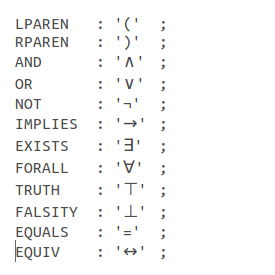
\includegraphics[scale=0.5]{tokens.png}\\
Together, the rules above represent the entire lexer file.

\section{Adaptor}
At this point we can return to look at the LogicTree class constructor which 
works as an adaptor for the parse tree. Antlr provides a user basic interface 
which can be run from the terminal to visualise this tree. For the sentence 
\emph{All men are mortal} the following tree will be generated:
\newpage
\begin{figure}[h!]
\centering 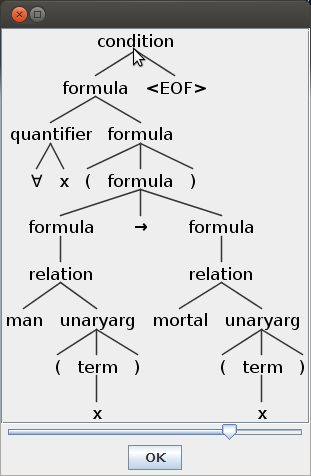
\includegraphics[scale=0.5]{antlr.png}
\end{figure}
\noindent Each node is created from one of the parser context classes. 
These are: 
\begin{verbatim}
folParser$ConditionContext
folParser$FormulaContext
folParser$QuantifierContext
folParser$RelationContext
folParser$BinaryargContext
folParser$UnaryArgContext
folParser$TermContext
\end{verbatim}
The first thing to notice is that the parser will generate a \emph{formula} node 
that does not correspond a type of logic node but is just a rule that guides the 
parsing. For this reason I created the dummy node which simply points to the 
rest of the tree through a LogicTreeNode field and returns that node's outcome 
without altering it.
\\ \\  
The adaptor provides a rule of interpretation for each of these classes through 
a switch statements. The default case is an error message for a complete 
picture, although it is not reachable, as each node of the parse must be an 
instance of one of these classes. The constructor performs a breadth first 
search and generates the appropriate LogicTreeNode for each node in the parse 
tree. Once finished it returns a pointer to the head of the tree. 
\\ \\
It is important to mention that in order to create the unary and binary relation 
nodes the adaptor keeps track of quantified variables in order to prevent the 
creation of a relation with an unbound variable as argument. In this way the 
tree is created only if the formula does not contain any free variables and so 
is a sentence and can be evaluated. Otherwise the user will be prompted to 
revise their input.

\section{User Interface}
With the process of creating a logic sentence from a raw string input concluded, 
we can now take a look at how the user can use this to understand semantics. 
This is how the workbench looks like, with the designed such that the sentence 
\emph{All men are mortal} evaluates to true:
\begin{figure}[h!]
\centering 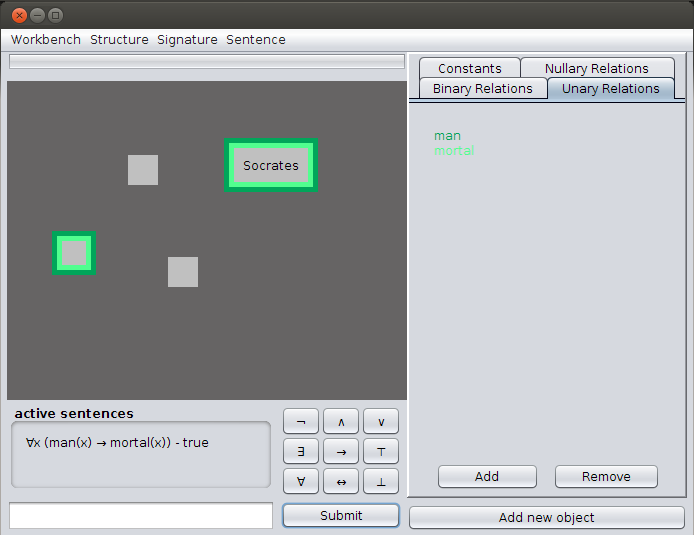
\includegraphics[width=\textwidth]{workbench.png}
\end{figure}

\subsection{The View}
The layout of the workbench is also designed around the three main elements 
involved in semantics:

\begin{enumerate}
\item \textbf{Structure panel} \\
This represents the main working area, taking up most of the upper left side, 
with a background of a darker grey than the rest of the workbench. It contains 
the following elements:

\begin{itemize}
\item Objects \\
The light grey squares represent objects in the structure and are labelled with 
the name of the constant that refers to them, otherwise are left blank. In this 
case Socrates describes the upper right square. The squares can be dragged, 
deleted, renamed and different relation symbols can be applied to them. \\
Objects are built from the Blob class. To make objects draggable, I implemented 
a mouse listener that overrides the MouseDragged method such that when it 
detects this behaviour it resets the location of the object to where the cursor 
is, however limiting its movement to the bounds of the structure panel. \\
A new unlabelled object can be added using the button at the bottom right of the 
screen. Deleting an object refreshes the active sentence list, deletes any 
relation symbols related to it and if it is a constant any sentence that 
contains it is also deleted. At least one object must be present in the 
structure at all times. If there is only one left the user is not allowed to 
remove it.

\item Unary relation symbols \\
These relations are represented by coloured borders around the objects they 
apply to. Furthermore, with a right click on an object the user can see a list 
of the unary relations names with a tick indicating which ones apply. This menu 
allows the user to change if a unary relation applies to an object or not. The 
relations are colour coded. In the example above Socrates is described by the 
relations man and mortal and as such has two coloured borders. \\
Unary relations are not created from a class, they are simply borders. In order
to add multiple borders the controller uses a CompoundBorder on objects and the
'colours' field of the object which is an array of the colours that must be
visible. These colours are added by the controller in the UpdateStructure method
at the start and is are updated on every relevant change.

\item Binary relation symbols \\
These relations are represented by arrows. If an arrow exist between two object, 
a list of names labels the arrow indicating which relations exist between the 
two. The list is situated near the second argument, next to the arrow head, such 
that the user can clearly see two arrows if there are relations going both ways. 
In the following example the object named by Fred loves the object named by Tina 
and vice versa, Fred believes in Tina and Tina loves herself.
\newpage
\begin{figure}[h!]
\centering 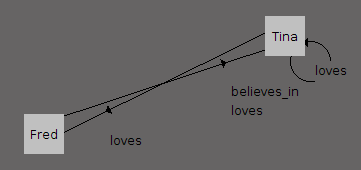
\includegraphics[scale=0.7]{arrows.png}
\end{figure}

Arrows are built from the Arrow class, designed to override the paintComponent 
method such that they follow the objects around as they are being dragged. To
do this the arrow class has Blob fields 'to' and 'from' and uses their
coordinates to draw the line between the two. As the paintComponent method is 
called every time a change occurs, the arrow will be redrawn when objects
are dragged.\\
For the arrow head, a polygon object is used along with a transition which
ensures the arrow is always pointing towards the object representing the second
parameter of the binary relation.

\item Nullary relation symbols \\
These come up at the bottom left side of the structure panel as they are added. 
Their default value is false and this is indicated by their names being faded 
out. A tool tip text also indicates this. To toggle their value the user can 
simply click on their names. These are also draggable, such that the user can 
decide how to make best use of the space available. \\
Nullary relations are built from the Blob class, with the right click 
functionality removed and the right click functionality added. This is to make
use of the mouse adaptor that makes these objects draggable.

\begin{figure}[h!]
\centering 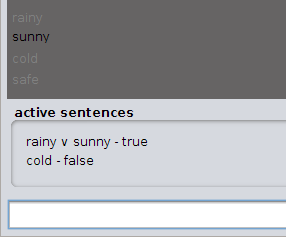
\includegraphics[scale=0.6]{nullary.png}
\end{figure}

\end{itemize}

\noindent The structure panel is resizeable and scrollable for a more 
comfortable user experience.

\item \textbf{Signature panel} \\
This is the tabbed panel at the right side of the workbench, with a tab for each 
type of element: constants, nullary, unary and binary relation symbols. Each 
tab also contains buttons for manipulating their content.

\begin{figure}[h!]
\centering 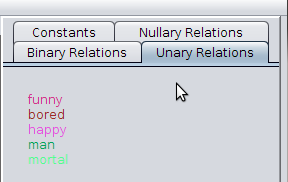
\includegraphics[scale=0.7]{signature.png}
\end{figure}

\noindent Constants can be removed, added or renamed. In the case of the second 
two actions, a text field appears such that the user can choose the desired 
name. Furthermore, in the case of renaming and removing, a constant must be 
selected from the list, otherwise the user is prompted accordingly. 
\\ \\
Unary relations are the only ones colour coded. Their name colour in the 
signature corresponds to a border colour in the structure. To generate an unique 
colour for each I used their name's hash code. To display this in the unary 
relation tab, I wrote a cellRenderer class for the list to use. Relations can be 
added or deleted. If the latter is performed, all corresponding borders are 
deleted along with any sentence that uses it. 
\\ \\
In addition to this, the binary relation tab has got a \emph{choose parameters} 
button. To use it, one of the relations in the list must be selected. Once 
pressed the button turns red and the user is prompted to click on two objects 
subsequently. To clear the selection the user can click on an empty area in the 
structure. Once the objects have been chosen an arrow is added (or a name to the 
list of labels if an arrow is already present) and the button returns to its 
original colour. 
\\ \\
Finally, the nullary relations tab also provides buttons for adding, renaming or 
removing a relation from the structure.

\item \textbf{Sentence panel} \\
Situated at the bottom of the window, it provides the means for introducing 
logic formulas and a scrollable list to store them and their outcome. Buttons 
are provided for the logic symbols along with a text field for the input and a 
submit button. The user will be prompted in case of bad input as accurately as 
possible.
\\ \\
The sentence list is refreshed every time a change occurs in the 
structure. However the user can use the menu to manually refresh it if they 
wish to do so. The list of active sentences ensures the last indexed sentence 
is visible. 
\\ \\
The user can also load text files containing sentences into the active sentence
list on the sentence panel. These will be automatically evaluated if they are 
valid for the active structure, otherwise ignored. The purpose of this is to
be able to provide some examples for students to examine and get familiar with
how the application works.\\
\begin{figure}[h!]
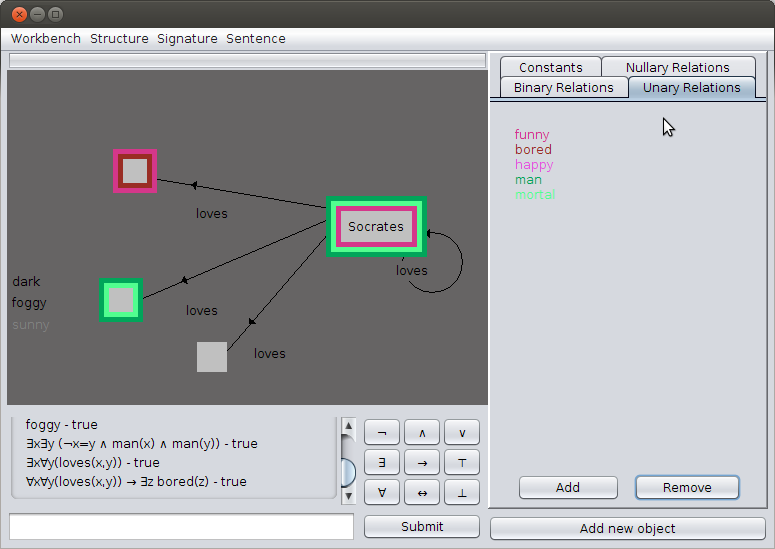
\includegraphics[width=\textwidth]{socratesSentences.png}
\caption{A number of sentences evaluated in the Socrates structure}
\end{figure}
\end{enumerate}

\subsection{The Tutorial}
The program comes with a set of questions the user can choose to bring up and
answer. They come up on a panel above the sentence box. The user can try and
answer, then, when they decide they have done so, move on to the next one.
This feature is at this moment very basic as it came on top of the essential
functionality and there was little time left. But it can still guide the users
and give them ideas as to what to practice on. More such questions can easily
be added. \\ \\
This is how the quiz looks like:
\begin{figure}[h!]
\centering 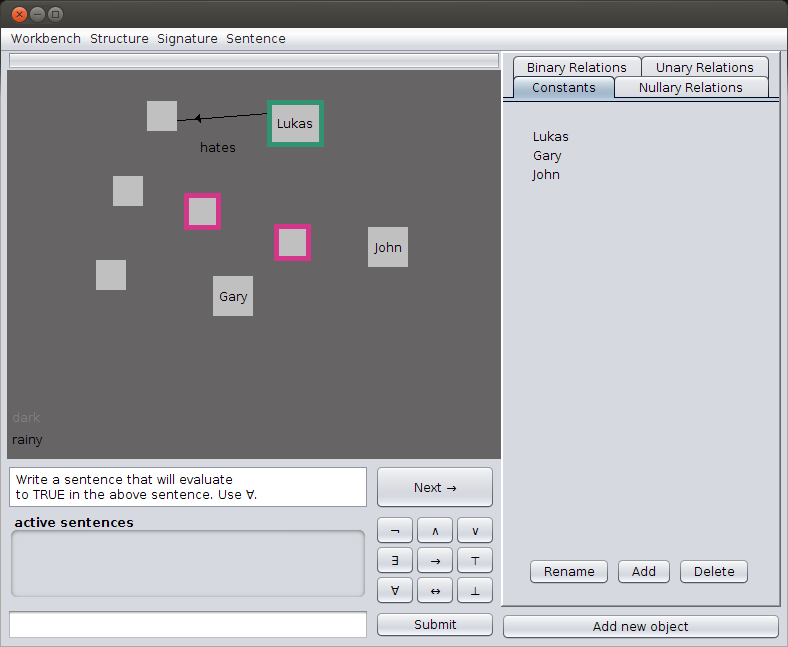
\includegraphics[width=\textwidth]{quiz.png}
\end{figure}

\section{The Controller}
So far, the display contains a series of components. However, in order to have 
any meaning, they must be linked to the Structure and Signature described in the 
evaluator. This is the role of the controller.
\\ \\
To link the signature panel to the signature class is uses a list model for each 
of the tabs and ensures a consistency between the relations and constant names 
in displayed and the ones present in the signature object. List models can be 
modified dynamically so they serve this purpose well.
\\ \\
To link the structure panel to the structure class it uses two pairs:
\begin{verbatim}
Pair<Term, Blob>
Pair<BinaryRel, Arrow>
\end{verbatim}
There is no pair for unary relations to borders as the link is simply the colour 
generated with the name's hash code. Along with a method to update the 
structure, the controller ensures a permanent consistency between the 
structure's fields' content and the panel.
\\ \\
To link the sentence panel to the logic tree, the controller uses the Antlr 
library to first parse the input and generate a parse tree, then uses the 
constructor in the LogicTree class to verify and build the sentence. After this 
it calls evaluate on the head of the logic tree and adds the outcome along with 
the sentence to the sentence list. When this is done it clears the quantified 
variables from the sentence scope such that the next sentence can start fresh.
\\ \\
Finally the controller provides methods to link actions described by the buttons 
on the screen to their desired effect in the structure and signature objects.
\\ \\
The following UML diagram\cite{uml} summarises the interface package: \\
\begin{figure}[h!]
\centering 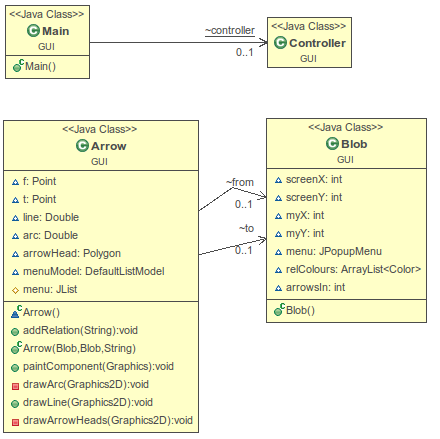
\includegraphics[scale=0.7]{gui.png}
\end{figure}

\section{Exception handling and user guidance}
Even the most intuitive interface needs to be able to guide its user if 
necessary. This is done mainly with the help of useful error messages. There is 
also some user guidance provided through the menu bar at the top of the screen. 

\subsection{Menu bar}
There are four menus at the top of the window:

\begin{figure}[h!]
\centering 
\includegraphics[scale=0.6]{menu.png}
\end{figure}

\begin{itemize}
\item Workbench \\
Provides the functionality needed for saving and loading an entire session 
comprising of the signature, structure, sentence list and progress made with the 
tutorial. It also allows choosing whether to display the question panels.\\
The account and preferences items have not yet been implemented, however they 
are intended for the user to be able to customize their experience. This will 
be discussed in the evaluation section. \\
At the bottom of this menu there is a help option which brings up a window with 
basic, concise instructions and a link to further first order logic information 
(i.e.\ the Wikipedia page for first order logic).

\item Structure \\
This menu provides functionality for saving and loading just the structure 
state. It offers an option to generate a new random structure which will replace 
the active one, as only one structure can be active at a time. \\
In order to save the structure to a file, I made use of object serialization. 
Every class involved in the structure implements Serializable for this purpose. 
When saving is performed, a file chooser is brought up such that the user can 
choose where to store the file along with a name for it. If the structure had 
already been saved and was just modified, the saving will overwrite the same 
file unless the user chooses the 'save as' option. Next, an object stream 
(ObjectOutputStream) is opened to the file. Then the Structure object is written 
to that stream. Finally, the file is closed (which also closes the object output 
stream). \\
Loading is performed in the reverse order. The user chooses a file with the file
chooser (JFileChooser), an object input stream is opened from the file and the
object is read. Once read it can be cast back to its original class. The file is
then closed (this will reset the pointer back to the start of the file so that
it can be used again in the future).

\item Signature \\
As it is strongly related to the structure and updated according to its content 
there are not a lot of things one can do with it. For this reason the only 
option is whether to show or hide the panel.
\item Sentence \\
This menu provides options for refreshing or clearing the sentence list, as well 
as for loading a sentence file. The format of such a file is plain text, with a 
sentence on each line. Once loaded they will be evaluated and placed in the 
active sentences list. If it fails to do so (the sentence may be using symbols
not defined in the structure for example) it simply ignores them and moves on.
\end{itemize}

\subsection{Error messages}
In order to handle bad user input or illegal operations I designed a number of 
exception classes. These prompt the user with regards to their logic sentence 
input.

\begin{itemize}
\item DuplicateDefinitionException\\
It is thrown during the creation of the logic tree if a second quantifier 
attempts to bind an already quantified variable.
\begin{figure}[h!]
\centering 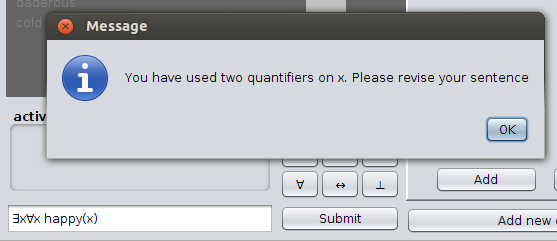
\includegraphics[scale=0.6]{duplicate.png}
\end{figure}

\item UnboundException\\
It is thrown if the LogicTree constructor attempts to create a unary or binary 
relation node using an unbound variable as argument for the node's relation. It 
may also be thrown if the user tries to use the name of a Constant that does not 
exist.
\newpage
\begin{figure}[h!]
\centering 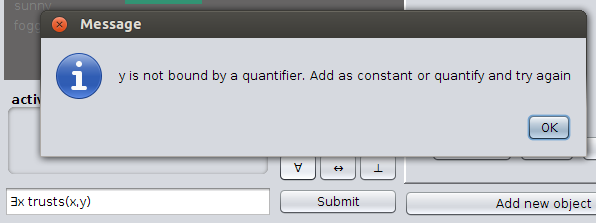
\includegraphics[scale=0.6]{unbound.png}
\end{figure}

\item UndefinedRelationException\\
It is thrown if the LogicTree constructor attempts to create a relation node 
with a name that the signature does not contain. The same type of notification
is brought up on the screen.
\begin{figure}[h!]
\centering 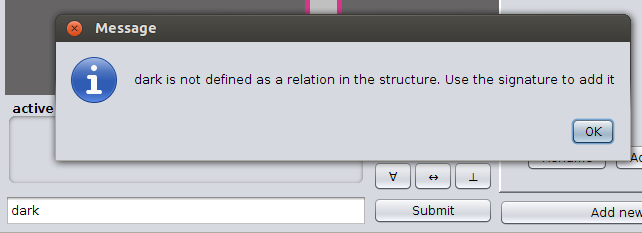
\includegraphics[scale=0.6]{undefrel.png}
\end{figure}

\end{itemize}

\noindent Some further assistance is provided using default Java exceptions:
\begin{itemize}
\item Index out of bounds\\
This can occur when a user presses buttons that require a list element to be 
selected so that the method can pass down an index. In such cases an error 
message is displayed only once to instruct the user that they must make a 
selection.
\item I/O exception\\
This can occur when the user tries to load a corrupted or otherwise inaccessible 
file. The error message informs accordingly.
\end{itemize}

\noindent Finally some guiding messages are displayed depending on the user's 
intention:

\begin{itemize}
\item If they want to add a binary relation a message tells them to click on two 
objects subsequent
\item If they want to add or rename a constant a message tells them they need to 
choose a name
\item If they want to load or generate a new signature a message asks them if 
they want to save the current signature
\end{itemize}

\noindent All these messages are only displayed once since it might otherwise 
become irritating for the user to keep having to click 'ok' when they want to, 
for example, add a constant.

%-------------------------------------------------------------------------------
%   EVALUATION
%-------------------------------------------------------------------------------

\chapter{Evaluation}
This section will try to provide an overview of what my solution to the project 
specification has achieved by relating it to existing solutions as well as my 
own expectations. I will use this opportunity to point out what is flawed or 
missing, as well as justify and explain why it is so.

\section{Quantitative evaluation}
My first priority was to make a minimum viable product that meets the project's 
compulsory requirements. These are as follows:

\begin{enumerate}
\item Notation should be as used in the course: Yes.\\
The formula field allows as valid input any sentence that respects first order 
logic syntax, making the brackets optional where possible. The lexer section 
describes how it allows the right names for relation, variable and constant 
names.

\item All aspects of the software should be controlled via a graphical user 
interface. It should be attractive robust, and easy to learn and use: Yes.
\\ \\
Although it is a subjective matter whether the interface is easy to use, the 
fact that it covers all aspects of the back end and provides complete 
functionality for modifying the structure and signature is verifiable.
\\ \\
I have also received some good feedback from two of my colleagues. I asked them 
to modify the structure such that the sentence \emph{All men are mortal} would 
be evaluated to true and then input the sentence for evaluation. They had no 
trouble in doing so. One tester did refer to the help menu, however just out of 
curiosity and admitted they would probably not use it.\\ As for its appearance, 
they found the program's simplicity pleasing and said it is quite comfortable. 
However they both had a reservation regarding the Swing look and feel which they 
considered a bit outdated. I agree the program should be customizable to use 
more modern skins and fonts. This is the intended purpose for the preferences 
item in the Workbench menu. However time did not allow it and it was quite low 
on my list of priorities.

\item The user should be able to create and edit signatures with up to at least 
6 constants, 3 unary relation symbols, and 3 binary relation symbols, and 
structures whose domains have up to at least 12 objects, all in the sense of 
the department's logic course: Yes.
\\ \\
I managed to implement the ideal case, where there are no limits on the number 
of objects or symbols. The program also uses a minimum number of arrows such 
that the work area does not become confusing. Although it does not automatically 
arrange the objects to a best distribution across the surface, it allows them to 
be rearranged by dragging, such that the user can decide what is most 
comfortable to them.
\\ \\
There is a basic alignment done across the diagonal of the structure area. 
Automatic uniform or otherwise better distribution would be a good addition, 
however the complexity of the algorithm was to high and could not be implemented 
within the time limit.

\item Users should be able to save structures to a file and load saved 
structures for further editing: Yes.
\\ \\
Structures can be saved and loaded locally on the user's computer. When loading 
a structure the signature is updated accordingly. In addition, the user can save 
the entire workbench consisting of the signature, structure, sentences and 
tutorial progress. 

\item The user should be able to create and edit first-order sentences. The 
software should display them correctly, with proper logical symbols for boolean 
connectives and quantifiers: Yes.
\\ \\
The interface displays a user friendly sentence format which is consistent with 
first order predicate logic syntax rules. It hides at all times the tokens used 
in the parsing process. 

\item The software should be able to correctly evaluate any first-order sentence 
in any structure of appropriate signature: Yes.
\\ \\
When developing the evaluator at the start of this project, testing was quite 
difficult as input was only possible via the terminal. My understanding of the 
bigger picture was not yet perfect. This only came after writing the interface 
and implementing the model-view-controller design. Separating the back end from 
the interface played a crucial role in allowing me to make changes, debug and 
simplify the back end code, whilst the interface allowed me to more easily input 
sentences for testing. 
\\ \\
It was only towards the end of the project that I managed to fix some of the 
evaluation bugs such as the asymmetry of the parameters for binary relations and 
the equals operator. In the end, I managed to half the size of the code for the 
logic tree and simplify the process of assignment passing to an easily readable 
implementation. I even removed one of the exception classes as it became 
obsolete. Although it might be very tempting for one to consider a part of their 
development finished, revising it after the entire thing is done will inevitably 
improve it as it will interact better with the rest of the software.
\\ \\
Within a structure containing the binary relation R, the unary relation P, the 
nullary relations A, B, C and constants Fred and Tina, I evaluated the following 
sentences, changing the situation to make them true and false subsequently. The 
evaluator has performed correctly in every case:
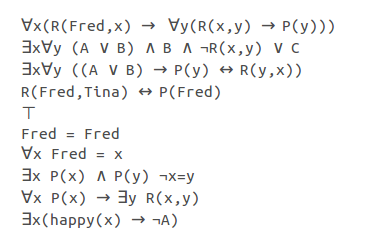
\includegraphics[scale=0.5]{testing.png}

\item The software should be able to lead the user interactively through the 
evaluation, along with comprehensive help facilities: No. 
\\ \\
Although the program provides a few basic tutorial questions, the tutorial tool 
cannot yet asses the student's performance. Unfortunately time was not 
sufficient to further develop this feature. As it is now, the student can read 
and answer the questions and mark the question as completed himself once he 
considers it is resolved. 

\item Several examples of structures and sentences should be provided: Yes.
\\ \\
The program automatically generates random structures. There is also a file 
provided with a number of example sentences which the user can load in the 
active sentence list. However at this stage the program will only load the 
sentences that are valid in the structure. A better approach would be for it to 
automatically add any constants and relation symbols it uses to the structure. 
\end{enumerate}

\section{Qualitative evaluation}
Qualitative aspects I feel are important to mention mainly concern the interface 
experience. This is relative to each user, however there are a two things that I 
am certain are satisfactory:
\begin{itemize}
\item Speed - throughout testing and general use the program has behaved very 
well, without crashing or delays. The buttons and menus are responsive and the 
overall experience smooth
\item Simplicity - counting the logic symbol buttons as a group, there are never 
more than 7 buttons visible on the screen at one time. This allows the user to 
focus on the structure and sentences, without having to worry about overwhelming 
toolbars. 
\end{itemize}

\noindent Of course there are also a number of improvements that can be made. 
Amongst these, the ones I consider most important are as follows:

\begin{itemize}
\item The ability to rename objects from the structure and add new binary 
relations directly from the structure: this would virtually eliminate the need 
for a signature panel as they are the only two actions that cannot be performed 
without it. It would further simplify the interface and provide a clean 
interaction. The user could the work with this:
\begin{figure}[h!]
\centering 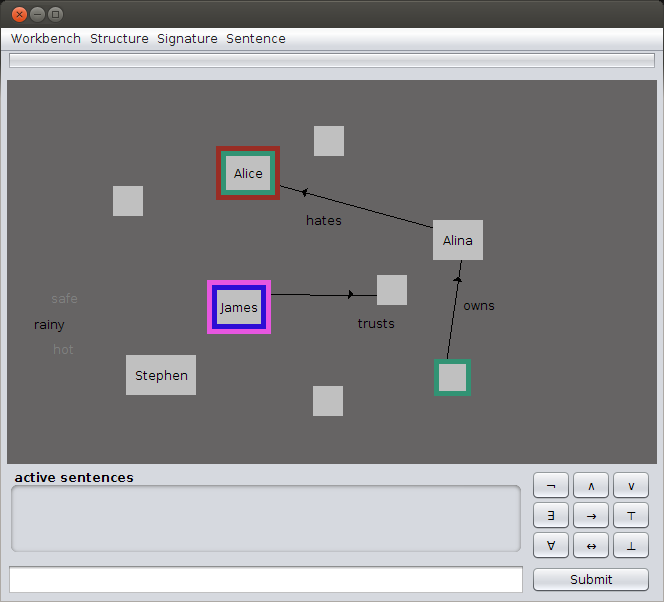
\includegraphics[scale=0.45]{simple.png}
\end{figure}

\item Provide better user feedback: as mentioned before my tutorial 
implementation is very basic because of time limitations. However user 
feedback is extremely important for keeping the student engaged and interested.
\item Progress bar: although it exists on the workbench, it is not correlated 
to the user activity. 
\end{itemize}

\section{Conclusions and Future Work}
With a full bug proof evaluator and all the essential functionality provided 
through the interface, this program could be the base of beautiful extensions. 
As mentioned before, one of them could be an implementation of the Hintikka 
game, which would contribute to the sense of satisfaction of the student as 
well as to their motivation to use the tool. 
\\ \\
I also consider it an important improvement that the application is made 
available online. This would would make it easier for the students to access the 
application and keep track of their progress, and would allow them to compare 
their performance to others.
\\ \\ 
For robustness, the tool should be linked to a lesson database accessible by
students and lecturers alike. The former should also have permissions to add,
edit or remove lessons and see their student's progress. I strongly believe
these three improvements would make a robust and truly useful teaching tool.
\\ \\
The time allocated for the project was sufficient for me to be able to gather
sufficient background information and get comfortable with the necessary tools.
It also allowed me to somewhat improve the minimum viable product. However for
it to be made into a complete teaching software which provides good feedback to
students, considerably more time would have been necessary. I am hoping the
current implementation will be considered as a starting point for improvements
and extensions by future students.
%-------------------------------------------------------------------------------
%   BIBIOGRAPHY
%-------------------------------------------------------------------------------

\begin{thebibliography}{9}
\bibitem{tarski}
  \emph{Tarski's World Support and Documentation}, \\
  OpenProof Software, \\
  http://ggweb.stanford.edu/support/manual/tarski

\bibitem{antlr4}
  Terence Parr, \\
  \emph{The Definitive ANTLR 4 Reference}, \\
  The Pragmatic Bookshelf, 2013

\bibitem{javaAPI}
  \emph{Java\textregistered Platform, Standard Edition 7, API Specification},\\
  Oracle, \\
  http://docs.oracle.com/javase/7/docs/api/index.html 

\bibitem{javaTUT}
  \emph{The Java\textregistered Tutorials}, \\
  Oracle, \\
  http://docs.oracle.com/javase/tutorial/index.html

\bibitem{compilers}
  Naranker Dulay, \\
  \emph{Compilers 221 lecture slides} \\
  https://www.doc.ic.ac.uk/~nd/compilers/

\bibitem{progit}
  Scott Chacon, \\
  \emph{Pro Git} \\
  http://git-scm.com/book

\bibitem{latex}
  \emph{LaTeX manual}, \\
  WikiBooks, \\
  http://en.wikibooks.org/wiki/LaTeX

\bibitem{logicslides}
  Ian Hodkinson, \\
  \emph{Logic 140 lecture slides}, \\
  http://www.doc.ic.ac.uk/~imh/

\bibitem{uml}
  ObjectAid, \\
  http://www.objectaid.com/

\end{thebibliography}

%-------------------------------------------------------------------------------
%   APPENDIX
%-------------------------------------------------------------------------------

\appendix
\chapter{Parser grammar}
\begin{verbatim}
grammar fol ;

condition
  : formula EOF ;

formula
  : TRUTH
  | FALSITY
  | term EQUALS term
  | relation
  | quantifier formula
  | NOT formula
  | formula AND formula
  | formula OR formula 
  | formula IMPLIES formula
  | formula EQUIV formula 
  | LPAREN formula RPAREN ;

term
  : VARIABLE
  | NAME ;

quantifier
  : FORALL VARIABLE
  | EXISTS VARIABLE ;

relation
    : NAME binaryarg
    | NAME unaryarg
    | NAME ;

binaryarg
    : LPAREN term ',' term RPAREN ;

unaryarg
    : LPAREN term RPAREN ;

\end{verbatim}


\chapter{Further Code UML Diagrams\cite{uml}}
\newpage

\begin{figure}[h!]
\centering 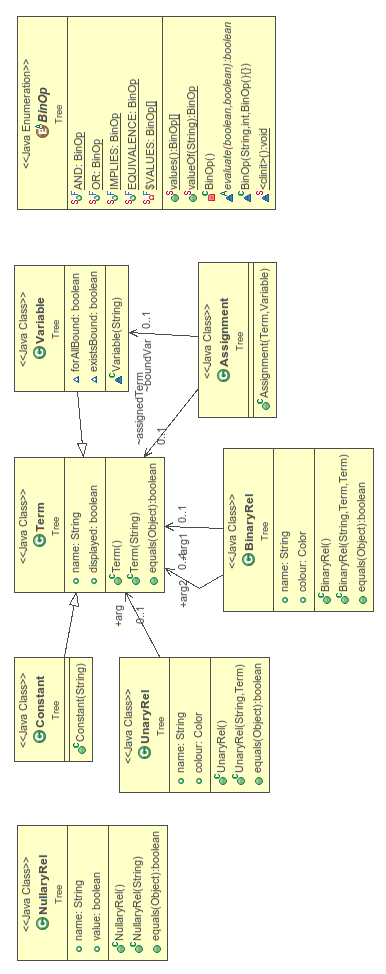
\includegraphics[height=\textheight]{treeBase.png}
\caption{Summarises the classes the logic tree is based on (fields of the logic 
tree nodes)}
\end{figure}
\newpage

\begin{figure}[h!]
\centering 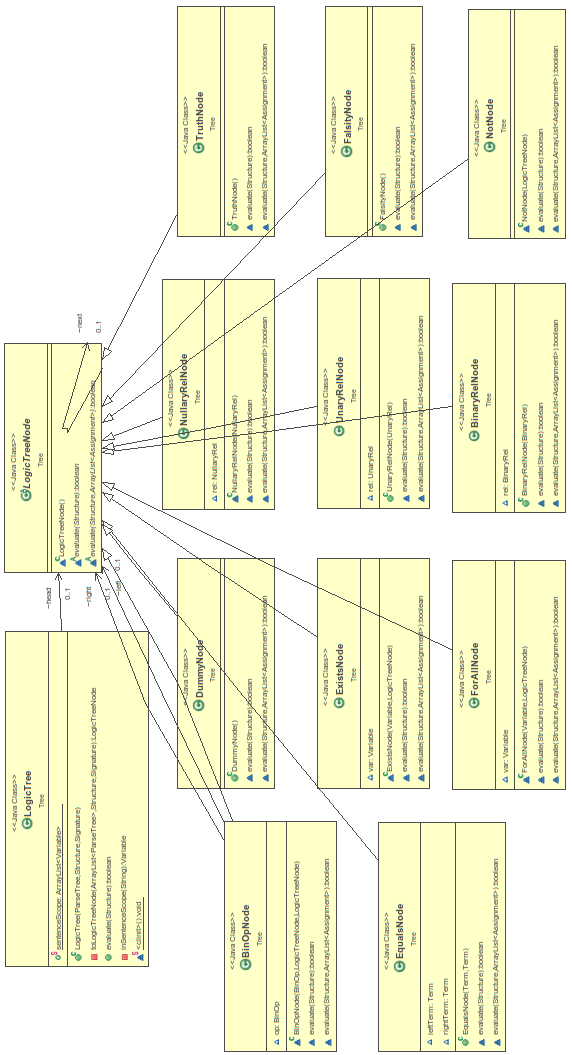
\includegraphics[height=\textheight]{treeNodes.png}
\caption{Summarises the LogicTree structure}
\end{figure}
\newpage

\newpage

%\chapter{Short demo}

%-------------------------------------------------------------------------------

\end{document}

% delete sentences that use deleted unary, binary, unary
% loading sentences
% question file
